\section{How to choose the symbols to use?}
\label{sec:choose}

It is important to realise that there are in general more than one way to represent a system in SBGN \PD. The choice of concepts and symbols often depend on the granularity of information available, and the message the authors of the map wish to convey to the readers of the map. 

As a first example of variable information granularity, let's take will take the example of MAP kinase phosphorylation (ERK). A very simple representation would be to encode the state of phosphorylation in \glyph{entity pools node} with different names, ERK, ERK-P, ERK-PP (\fig{MAPK-NoVar}).
 
\begin{figure}[H]
  \centering
  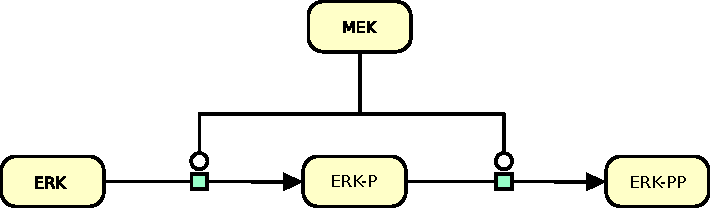
\includegraphics[scale = 1]{images/MAPK-NoVar}
  \caption{Phosphorylation of ERK by MEK, where ERK is represented by three different macromolecules.}
  \label{fig:MAPK-NoVar}
\end{figure}

This kind of representation would be obtained if the SBGN \PDm was generated from a model encoded in SBML core \cite{Hucka:2003}. One of the problems with this representation is the difficulty for the reader to understand that the effect of MEK is to catalyse the phosphorylation of ERK. A scientist familiar with signalling pathways would probably imediately make the connection. A biologist in general could be more cautious. ``P'' could represent anything (peptide? proline?). A computer would require a special algorithm to parse the names, and this algorithm would easily fail. Instead of ERK-PP, we could have used PP-ERK, ERK\_PP, ERKP1P2, ERKTPYP etc. But in fact, there is nothing in the the map \fig{MAPK-NoVar} indicating that the reactions catalysed add covalent modifications to ERK. Thore reactions could be anything, such as aggregation, cleavage etc.

In order to overcome those issues, one can use state variables. On \fig{MAPK-OneVar}, one uses a single state variables to represent the number of phosphorylations on ERK. 

\begin{figure}[H]
  \centering
  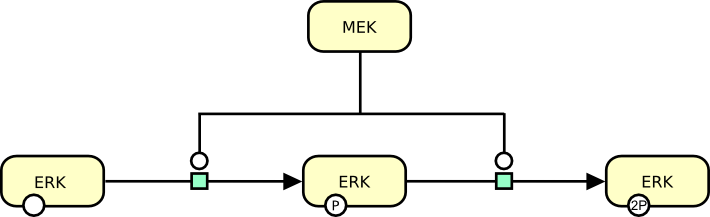
\includegraphics[scale = 1]{images/MAPK-OneVar}
  \caption{Phosphorylation of ERK by MEK, where ERK is represented by three different states, non-phosphorylated, mono-phosphorylated and bi-phosphorylated.}
  \label{fig:MAPK-OneVar}
\end{figure}

Because 'P' is a reserved symbol of the covalent modifications vocabulary, there is no ambiguities. We know that each reaction add a phosphate to ERK. That would be the representation to favour if we only know the number of phophorylation (e.g. by western blot with non-specific antibodies), or if we do not care which site is phosphorylated. Note that the leftmost ERK carries an empty state variable, that is equivalent to ``0P''. The state variable is not ommited. This rule of \SBGNPDLone is called ``once a variable, always a variable'' (OVAV).
If we want to, or can, be more specific about distinct phosphorylations, one can create two state variables, one for each site (\fig{MAPK-TwoVar}). 

\begin{figure}[H]
  \centering
  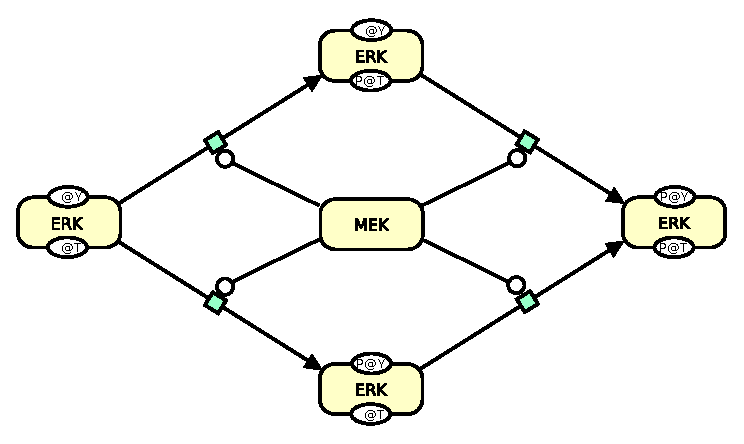
\includegraphics[scale = 1]{images/MAPK-TwoVar}
  \caption{Phosphorylation of ERK by MEK, where each phosphorylated form of ERK is represented.}
  \label{fig:MAPK-TwoVar}
\end{figure}

In this representation, we have all the information related to the two phosphorylation sites, the threonine and the tyrosine. They are represented by the variable symbols T and Y in the figure. But one could have chosen X and Y or 1 and 2. The important issue is to distinguish them. Note that the creation of an extra \glyph{entity pool node} is unavoidable. \SBGNPDLone does not currently allow logical expressions in the state variables. Therefore if only one \glyph{entity pool node} was to be used to represent the single-phosphorylated form, a choice between T or Y should have been made, and the resulting map would not have carried the same information than  (\fig{MAPK-OneVar}).

% complex: macromolecule or complex
As a second example, we will consider the oxygenation of hemoglobin. If one wants to convey the message that 4 oxygene molecules bind to a molecule of hemoglobin, it is sufficient to create \glyph{macromolecules} for hemoglobin and oxy-hemoglobin. 

\begin{figure}[H]
  \centering
  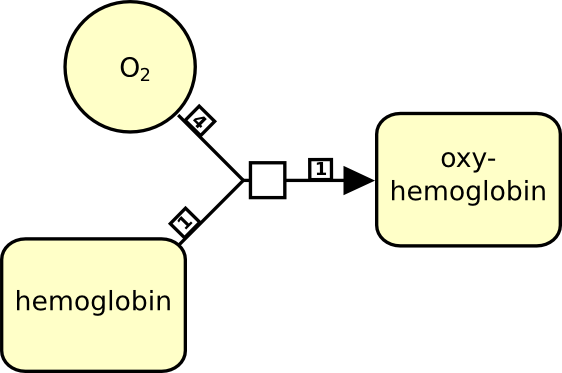
\includegraphics[scale = 0.4]{images/hemoglobin-macromolecule}
  \caption{Hemoglobin oxygenation using \glyph{macromolecules}.}
  \label{fig:hemoglobin-macromolecule}
\end{figure}

If conveying the fact that hemoglobin is a multimer is important (for instance to suggest cooperativity), one can use \glyph{multimers} instead. In addition, in \fig{hemoglobin-multimer}, the concept of oxygenation is represented with a state variable rather than being embedded in the name of the nodes.

\begin{figure}[H]
  \centering
  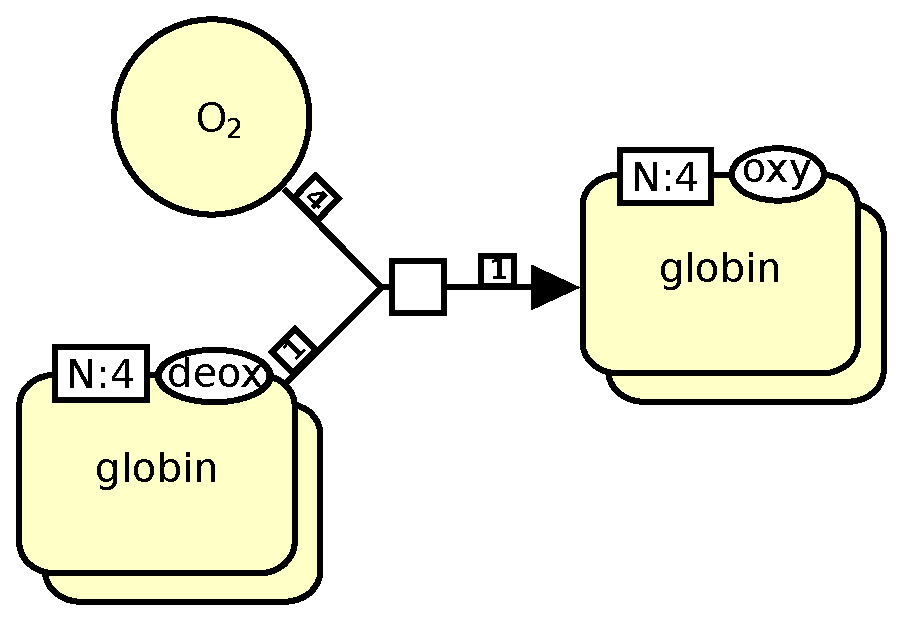
\includegraphics[scale = 0.4]{images/hemoglobin-multimer}
  \caption{legend}
  \label{fig:hemoglobin-multimer}
\end{figure}

An additional layer of complexity is needed if we want to mention the $\alpha$ and $\beta$ subunits. A \glyph{complex} can then be used. In addition \fig{hemoglobin-complex} explicitely represent the complexes between globin and oxygene instead of using state variables.

\begin{figure}[H]
  \centering
  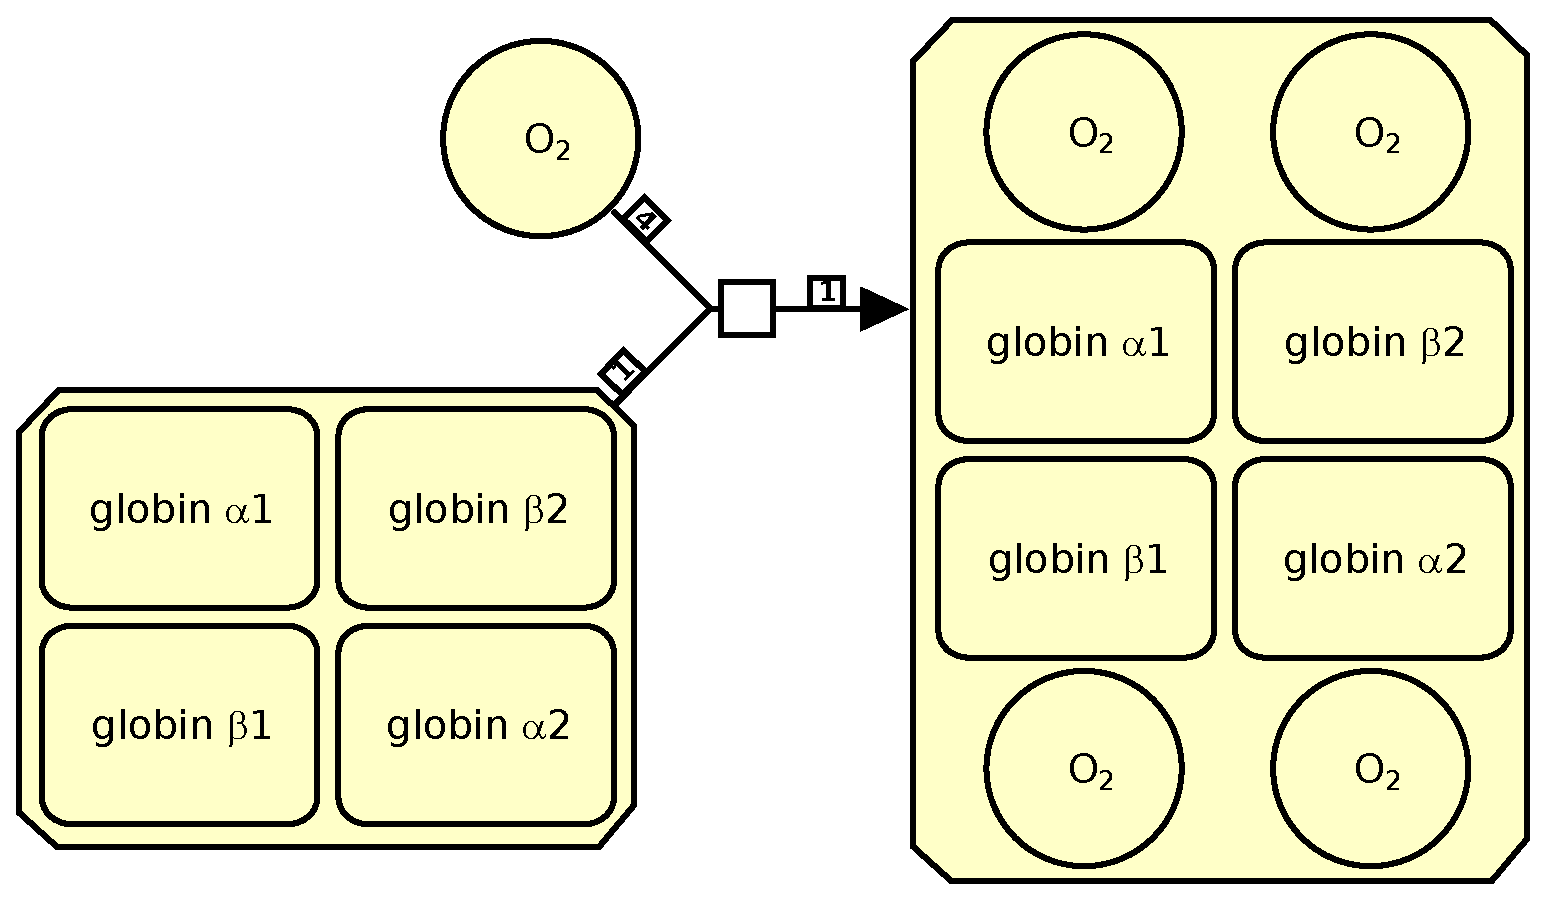
\includegraphics[scale = 0.4]{images/hemoglobin-complex}
  \caption{legend}
  \label{fig:hemoglobin-complex}
\end{figure}

In conclusion, one can see that many different choice are offered to represent an idea in SBGN, and the map writers make the choice. By doing so, they acknowledge that more or less information can be extracted from the resulting map. The important issue is that anyone reading the map interpret it the same way. That is the topic of the following section. 
